% !TEX encoding = UTF-8 Unicode
% !TEX spellcheck = en_US

\documentclass[a4paper, 11pt]{article}

\usepackage{nag}
\usepackage[utf8]{inputenc}
\usepackage[T1]{fontenc}
\usepackage{lmodern}
\usepackage[margin=2cm]{geometry}
\usepackage{enumitem}
\usepackage{fancyhdr}
\usepackage{natbib}
\usepackage{caption}
\usepackage{subcaption}
\usepackage{lastpage}
\usepackage{amsmath}
\usepackage{graphicx}
\usepackage{xcolor}
\usepackage{hyperref}
\usepackage{bibentry}
\usepackage{siunitx}

%% Specific commands
% the only place to specify version number (for consistency) - the date is the last modif for the code
\newcommand{\version}{1.10.00 (2023-04-06)}
\newcommand{\FullSWOF}{FullSWOF\_2D}
\newcommand{\FullSWOFUI}{FullSWOF\_UI}
\newcommand{\contactFullName}{The FullSWOF development team}
\newcommand{\contactFS}{\href{mailto:fullswof.contact@listes.univ-orleans.fr}{fullswof.contact@listes.univ-orleans.fr}}
\newcommand{\MainWebSite}{\url{https://sourcesup.renater.fr/projects/fullswof-2d/}}
\newtheorem{rmk}{Remark}

% Command to avoid a warning as some bibtex entries are written several times (ex: Delestre17 in the "how to cite" section and in the biblitography)
\makeatletter
\renewcommand\bibentry[1]{\nocite{#1}{\frenchspacing
     \@nameuse{BR@r@#1\@extra@b@citeb}}}
\makeatother


% Headers and footers
\lhead{\FullSWOF{} v\version}
\rhead{MAPMO-IDP --- INRAE}
\cfoot{\thepage{}/\pageref{LastPage}}
\pagestyle{fancy}

% Lists: spacing between items
\setlist{noitemsep, topsep=0pt, partopsep=8pt}

% URL style = normal
\urlstyle{rm}

% Unit style
\sisetup{%
	per-mode=symbol
}


\title{Documentation of \FullSWOF\\v\version}

\author{\contactFullName}%, \contactEmail}
\date{2023-01-26} % Last modif for the documentation

\begin{document}

\maketitle

\thispagestyle{fancy}

\tableofcontents

\section{Presentation of the \FullSWOF{} software}

The name \FullSWOF{} stands for ``Full Shallow Water equations for Overland Flow in two dimensions of space''.
In this software, the Shallow Water (or Saint-Venant) equations are solved using finite volumes and numerical methods especially chosen for hydrodynamic purposes (transitions between wet and dry areas, small water heights, steady-state preservation\textellipsis).
A graphic user interface is available at \url{https://sourcesup.renater.fr/projects/fullswof-ui/}.

For explanations concerning the numerical schemes and approximations, the reader is referred to \citet{Delestre14}, \citet{Delestre10b}, \citet{Delestre09} and \citet{DelestreJames09}.
For a precise description of the structure of the software in several classes, see the Doxygen file (\textsf{refman.pdf} in the \textsf{doc} directory) and~\citet{Delestre08}.
The structure  of the source code is designed to make future evolutions easy: for example, a new friction law can easily be added in the \textsf{libfriction} library, by creating a new friction file.

If you plan to change the code of \FullSWOF, see Section~\ref{sec:dvp} for explanations on how to use the benchmarks.
Doing so, you should pay attention to the license (Section~\ref{sec:license}).

\section{Software distribution}

\subsection{How to download \FullSWOF}
The \FullSWOF{} software can be downloaded on the website \MainWebSite.

\subsection{How to cite \FullSWOF}

The \FullSWOF{} software must be referred as:
\begin{quote}
	\nobibliography*
	\bibentry{Delestre17}.
\end{quote}

To improve the reproducibility of your results, we advise you to mention in your publication the version of \FullSWOF{} you used.

\subsection{License}\label{sec:license}
This software is distributed under CeCILL-V2 (GPL compatible) free software license.
So, you are  authorized to use the Software, without any limitation as to its fields of application.

If you make changes to \FullSWOF{} code, you are welcome to \textbf{contribute your changes to the main repository}, directly through the website (\MainWebSite) or by contacting its main developers (\contactFS).
You may prefer to distribute yourself the \emph{modified software}.
In such a case, we ask you to \textbf{change its name} in order to avoid confusion between your software and the original one.
In such a case, pay attention to the text that follows.

The license authorizes you to distribute a \emph{modified software}, in source code or object code form, provided that said distribution complies with all the provisions of the \emph{Agreement} and is accompanied by:
\begin{itemize}
	\item a copy of the Agreement,
	\item a notice relating to the limitation of both the Licensor's warranty and liability,
\end{itemize}
and that, in the event that only the object code of the \emph{modified software is redistributed}, you allow future users \emph{to access the full source code of the modified software by indicating how to access it}, being understood that the additional cost of acquiring the source code shall not exceed the cost of transferring the data.

For further explanation about this free software license, you should read the following links:
\begin{itemize}
	\item \url{https://cecill.info/licences/Licence_CeCILL_V2-fr.html} (in French)
	\item \url{https://cecill.info/licences/Licence_CeCILL_V2-en.html} (in English)
\end{itemize}
\subsection{Installation}
\begin{rmk}
	To windows' users: please, look at the application note entitled ``\href{https://sourcesup.renater.fr/docman/view.php/895/3949/AppNote-windows.pdf}{Using Cygwin to compile and run  \emph{FullSWOF\_1D}, \FullSWOF{} or \emph{SWASHES} under windows}''.
\end{rmk}

First unzip the archive of the software.
Go to the \FullSWOF{} directory, and write the following command lines:
\begin{quote}
	\textsf{make distclean}\newline
	\textsf{make}
\end{quote}
\begin{rmk}
	If you are on a multi-core machine, you can speedup the compilation by adding \textnormal{\textsf{-j N}} to your make command (where \textnormal{\textsf{N}} is the number of cores you want to use), like \textnormal{\textsf{make -j 4}} for using up to 4~cores.
\end{rmk}

For getting use with \FullSWOF, you could go to the \textsf{Examples/Simple} directory.
You will find a basic set of inputs file and launch your first flow simulation with \FullSWOF\@:
\begin{quote}
	\textsf{cd Examples/Simple}\newline
	\textsf{../../bin/FullSWOF\_2D}
\end{quote}

\subsection{Check for proper functioning}\label{sec:functionOK}
\FullSWOF{} comes with a set of test cases used for benchmarking (see Section~\ref{sec:valid}).
In the \textsf{Benchmarks} directory, each test case has its own directory, which initially contains:
\begin{itemize}
	\item the analytic solution (file \textsf{analytic.dat}),
	\item the \FullSWOF{} input parameters (\textsf{Inputs} directory)
	\item the statistics of the benchmark outcome, as computed by the developers (file \textsf{comp\_STANDARD.dat}).
\end{itemize}
Once the software is installed on your computer, it is worth checking its proper functioning.
For this, and assuming your operating system is 64~bits, simply run the command \textsf{make benchref} (or \textsf{make -j 4 benchref} to use four cores).
This will first compile a version of \FullSWOF{} adapted to the benchmarks (it is compiled with specific compilation flags for reproducibility).
Then all the test cases will be computed (the results of the computation will be stored in the \textsf{Outputs\_REFERENCES} directories) and the differences with the analytic solutions will be calculated.
Finally, it will be checked if there are differences between your run (called References) and the one of the developers (called Standard).
It is expected no such difference will be found: hence, for each test case, you should get the diagnosis ``Results are identical.''.
Otherwise, please, contact the developers at {\href{mailto:fullswof.contact@listes.univ-orleans.fr}{fullswof.contact@listes.univ-orleans.fr}}.

\begin{rmk}
	In benchmarking mode (\textnormal{\textsf{make benchref}} and \textnormal{\textsf{make benchuser}}, see Section~\ref{sec:make}), \FullSWOF{} compilation makes use of a specific option (\textnormal{\textsf{{-}{-}float-store}}).
	This improves the reproducibility of the computations but also double the computation time.
	The release mode (\textnormal{\textsf{make}}) does not use this option.
	This speeds up the computations but causes a slight decrease in the accuracy.
	In practical terms, this loss of accuracy should not have any consequences.
\end{rmk}

\section{Input and output values}
\begin{rmk}
	\FullSWOFUI{}, a graphic user interface dedicated to \FullSWOF{}, is available at
	\textnormal{\url{https://sourcesup.renater.fr/projects/fullswof-ui/}}.
\end{rmk}

\begin{rmk}
	To help you in getting the input data in the suitable format, and to make easier the processing of \FullSWOF{} outputs, the \textnormal{\textsf{Tools}} directory contains additional programs: conversion of a grid file (such as a DEM) in a GIS format (AscGrid) to the XYZ format expected by \FullSWOF{} (and vice-versa); extraction of a rectangular window from a XYZ file. To compile the files and get the binaries in the \textnormal{\textsf{bin}} directory, just run \textnormal{\textsf{make construction\_tools}}. 
\end{rmk}

\begin{rmk}
	If you are not comfortable with the concepts of CFL, numerical flux, linear reconstruction, etc., Section~\ref{rem:default} gives the input values we advise to use by default for overland flow.
\end{rmk}

When launched, \FullSWOF{} expects two subdirectories: one for the inputs, one for the outputs.
In the following sections, the notation \texttt{<x>} stands for the tag corresponding to the \(x\) variable, whereas the square brackets [\(\cdot\)] give the unit of the variable.

\subsection{\textsf{Inputs} directory}

You can set the values of most of the parameters in the \textsf{parameters.txt} file, located in the \textsf{Inputs} directory.

\subsubsection{Space and time scales}

First, you have to specify the \textbf{number of grid cells} \texttt{<Nxcell>} and \texttt{<Nycell>} (in space) and the \textbf{length of  the domain} along \(x\) and \(y\) (\texttt{<L>} [\si{\meter}] and \texttt{<l>} [\si{\meter}], respectively).
For the time, you should set the value of the \textbf{duration of the simulation} \texttt{<T>} [\si{\second}] and the \textbf{number of times saved} \texttt{<nbtimes>} (that is the number of ``pictures'' you will save to see the evolution as a movie).\newline
If you do not want to save pictures, you can set \texttt{<nbtimes>} to 0.

You can run \FullSWOF{} either with a \textbf{constant CFL} \texttt{<cflfix>} or with \textbf{constant time step} \texttt{<dtfix>}.
The type of time constraint is defined by \texttt<scheme\_type>.
You can choose either:
\begin{itemize}
	\item case~1: fixed CFL value.
	      You only have to specify the value of \texttt{<cflfix>}.
	      Usually, a CFL value equal to 0.4 is suitable.
	\item case~2: fixed time step (in seconds).
	      In this case, you have to specify the values of both \texttt{<dtfix>} and \texttt{<cflfix>}.
	      Indeed, it is always necessary to set the CFL value even if you choose the fixed time step because \FullSWOF{} verifies at each loop in time that the time step is not greater than this CFL value in order to respect the stability condition.
\end{itemize}

\subsubsection{Boundary conditions}
For each of the four boundaries (left, right, top and bottom), you have the choice between a constant boundary condition (in time and space) and an inhomogeneous boundary condition (in time and space).
For this, you have to fill the parameters \texttt{<L\_bc\_init>}, \texttt{<R\_bc\_init>}, \texttt{<T\_bc\_init>}, \texttt{<B\_bc\_init>} with:
\begin{itemize}
	\item case~1 to run \FullSWOF{} with an inhomogeneous boundary.
	\item case~2 to run it with a constant boundary.
\end{itemize}

For a constant boundary, you must specify the boundary type for the left, right, top and bottom boundary conditions using the parameter \texttt{<Lbound>}, \texttt{<Rbound>}, \texttt{<Tbound>} and \texttt{<Bbound>}, respectively.
The various types of boundaries are defined at the end of the section.

For an inhomogeneous boundary, you have to provide two kinds of files in the \textsf{Inputs} directory (Figure~\ref{Fig:BoundaryCondition}):
\begin{description}
	\item[A description of the evolution in time for the whole simulation.]
	      This file must contain two columns (fig.~\ref{Fig:BoundaryCondition:a}):
	      \begin{itemize}
		      \item the first column represents the time [\si{\second}].
		      \item the second column contains the name of the file describing the space configuration of the boundary (this second file is described below).
	      \end{itemize}

	      You have to specify the name of such a file in the parameters \texttt{<L\_bc\_NF>}, \texttt{<R\_bc\_NF>}, \texttt{<T\_bc\_NF>} and \texttt{<B\_bc\_NF>} (for the left, right, top and bottom boundaries, respectively).

	      Each column must contain at least one value.
	      The first value of the first column must be 0 (initial time).
	      If the file contains only one line (namely 0 in the first column and a file name in the second column), the boundary is constant in time during the run.
	      If the file contains several lines, the boundary will be changed during the run.
	      For example, let us consider a file with three values of time (\(0, t_1, t_2\)) and the corresponding three files for the boundary (\textsf{BC0.txt}, \textsf{BC1.txt}, \textsf{BC2.txt}, see next paragraph).
	      The boundary condition used will be:
	      \begin{itemize}
		      \item \textsf{BC0.txt} for \(0   \leq t < t_1\),
		      \item \textsf{BC1.txt} for \(t_1 \leq t < t_2\),
		      \item \textsf{BC2.txt} for \(t_2 \leq t\).
	      \end{itemize}

	      \begin{figure}[htbp]
		      \begin{subfigure}[b]{0.5\textwidth}
			      \centering
			      \begin{tt}
				      \begin{tabular}{ll}
					      \#time & file\_name \\
					      0      & BC0.txt    \\
					      120    & BC1.txt    \\
					      3600   & BC2.txt
				      \end{tabular}
			      \end{tt}
			      \caption{File of time evolution \textsf{BC\_time.txt}\label{Fig:BoundaryCondition:a}}
		      \end{subfigure}
		      %
		      \begin{subfigure}[b]{0.5\textwidth}
			      \centering
			      \begin{tt}
				      \begin{tabular}{llll}
					      \#x & c & q    & h      \\
					      0.1 & 2 &      &        \\
					      0.3 & 1 & 0.05 & 0.0005 \\
					      0.5 & 2 &      &        \\
					      0.7 & 3 &      &        \\
					      0.9 & 3 &      &        \\
					      1.1 & 3 &      &        \\
					      1.3 & 5 & 2.3  & 0.5    \\
					      1.5 & 5 & 2.3  & 0.5
				      \end{tabular}
			      \end{tt}
			      \caption{File of spatialization \textsf{BC0.txt}\label{Fig:BoundaryCondition:b}}
		      \end{subfigure}
		      \caption{Examples of files for the inhomogenous boundary conditions\label{Fig:BoundaryCondition}}
	      \end{figure}

	      \begin{rmk}
		      Be careful that the boundary condition may not change exactly at \(t=t_1\) but at \(t>t_1\).
		      Indeed, whether using a constant CFL or a constant time step, \(t_1\) might not be reached exactly.
		      We can have \(t<t_1\) for a given computing step, and the next computing step (at \(t+dt\)) may be greater than \(t_1\).
		      So, \(t=t_1\) may not be computed.
		      In this case, the change in boundary condition will take place at \(t+dt>t_1\).
	      \end{rmk}

	\item[The spatialization of the boundary for each range of time.]
	      This second type of file (which is named in the second column of the first type of file) describes the spatialization of the boundary condition (fig.~\ref{Fig:BoundaryCondition:b}).
	      It should be in ASCII, in the format ``\(x\) \(c\) \(q\) \(h\)'' (or ``\(y\) \(c\) \(q\) \(h\)'') in which \(x\) (or \(y\)) represents the coordinate along \(x\) (or \(y\)), \(c\) represents the type of boundary condition (see below), \(q\) represents the water discharge [\si{\cubic\meter\per\second}] and \(h\) represents the water height [\si{\meter}].
\end{description}
\medskip
For an example of using \FullSWOF{} with an inhomogeneous boundary condition, refer to the \textsf{Examples/Inhomogeneous\_boundary} directory.

\paragraph{The type of boundary condition is specified as:}
\begin{itemize}
	\item case~1 for the imposed height boundary condition (based on the modified method of characteristics).
	      \emph{Both discharge and water height} have to be specified (see below).
	      Depending on the regime (sub/super-critical) and on the flow direction (inflow or outflow), the value of the imposed discharge may be used or not by \FullSWOF\@;
	\item case~2 for the wall condition;
	\item case~3 for the Neumann boundary condition, which means that the normal derivatives of the water height and velocity are null (\textit{i.e.}\ no change in water height and velocity at the boundary).
	      Physically, this case is similar to an open boundary;
	\item case~4 for the periodic case, in which the outflow on one boundary is considered as the inflow on the opposite boundary.
	      In this case, at each time step, the incoming flow of one boundary is set equal to the outgoing flow of the other boundary;
	\item case~5, for an imposed discharge.
	      You must specify the value of flow discharge and the specific water height (see below), but the latter will be considered only in supercritical cases.
\end{itemize}
\medskip
For the imposed water discharge and height, you must use the following rules:
\begin{description}
	\item[Imposed discharges] \sloppy \texttt{<left\_imp\_discharge>}, \texttt{<right\_imp\_discharge>}, \texttt{<bottom\_imp\_discharge>} and \texttt{<top\_imp\_discharge>} [\si{\cubic\meter\per\second}] correspond to the discharges at the left, right, bottom and top boundaries, respectively.
	      At the left (\textit{i.e.} \(x=0\)) and bottom (\textit{i.e.} \(y=0\)) boundaries, if you want an incoming flow, you have to impose a \textit{positive} discharge whereas for an outgoing flow you must impose a \textit{negative} discharge.
	      \newline
	      At the opposite boundaries (\textit{i.e.} \(x=x_{max}\) and \(y=y_{max}\)), impose a \textit{negative} discharge
	      for the inflow and a \textit{positive} discharge for the outflow;
	\item[Imposed water heights] \texttt{<left\_imp\_h>}, \texttt{<right\_imp\_h>}, \texttt{<bottom\_imp\_h>} and \texttt{<top\_imp\_h>} [\si{\meter}] correspond to the water heights at the left, right, bottom and top boundaries respectively.
\end{description}

\begin{rmk}
	Be careful that the boundary conditions may not work as you expect!
	A careful testing is strongly advised, and some tweaking may be required to get what you want.
\end{rmk}

\subsubsection{Friction law}
You have to impose the \textbf{friction law} \texttt{<fric>}.
You can use either:
\begin{itemize}
	\item case~0 to run \FullSWOF{} with no friction.
	\item case~1 to use the Manning law.
	      The friction coefficient is the Manning friction coefficient [\si{\metre\tothe{-1/3}\second}].
	\item case~2 to use the Darcy-Weisbach law.
	      The friction coefficient is the Darcy-Weisbach friction coefficient [\si{dimensionless}].
	\item case~3 to use the Poiseuille law.
	      The friction coefficient is the Poiseuille friction coefficient [\si{\square\meter\per\second}], equal to the triple of the kinematic viscosity \(\nu\).
	      See \citet{Kirstetter16}.
\end{itemize}
If you choose case~1, case~2 or case~3, the value of the friction coefficient must be imposed either by using a file or by giving a value, according to the parameter \texttt{<fric\_init>}:
\begin{itemize}
	\item case~1 to load the friction coefficient from a file.
	      The file name is specified by the parameter \texttt{<fric\_NF>}.
	      This file must be in the \textsf{Inputs} directory.
	      It should be in ASCII, in the format ``\(x\) \(y\) \(f\)'' in which \(x\) represents the coordinate along \(x\), \(y\) represents the coordinate along \(y\) and \(f\) represents the friction coefficient.
	\item case~2 to use a constant friction coefficient over the whole domain.
	      This value is set by the parameter \texttt{<friccoef>}.
\end{itemize}
\begin{rmk}
	For a spatially variable friction coefficient, if the variation is too important (in particular if a discontinuity occurs), numerical errors such as spurious peaks may appear.
	A possible way to overcome this problem is to implement a well-balanced scheme for the friction source term, see for example~\citet{Bouchut04}.
\end{rmk}

\subsubsection{Numerical scheme}

\begin{rmk}
	For details about the numerical scheme, see \citet{Delestre14}.
\end{rmk}

The next six parameters are related to the numerical scheme.
You have to choose the:
\begin{description}
	\item[Numerical flux \texttt{<flux>}.] You can use either:
	      \begin{itemize}
		      \item case~1: Rusanov flux,
		      \item case~2: HLL (Harten, Lax and Van Leer) flux,
		      \item case~3: HLL2 flux, that is another way of programming HLL (unusual formulation but quicker resolution),
		      \item case~4: HLLC (Harten, Lax and Van Leer with Contact Surface) flux,
		      \item case~5: HLLC2 flux, that is another way of programming HLLC (unusual formulation but quicker resolution).
	      \end{itemize}
	      \begin{rmk}
		      The HLLC approximate Riemann solver is a modification of the basic HLL scheme to account for the influence of intermediate waves.
		      Indeed, the HLLC solver restores the missing contact and shear waves in the HLL scheme.
	      \end{rmk}
	\item[Order of the scheme\texttt{<order>}.] You can use either:
	      \begin{itemize}
		      \item case~1: order 1,
		      \item case~2: order 2.
	      \end{itemize}
	\item[Linear reconstruction \texttt{<rec>}.] This parameter will play a role only for a scheme of order~2.
	      It can be:
	      \begin{itemize}
		      \item case~1: MUSCL,
		      \item case~2: ENO,
		      \item case~3: a modified ENO\@.
	      \end{itemize}
	\item[ENO damping factor \texttt{<amortENO>}.] This parameter must be specified when you are using linear reconstructions ENO or modified ENO\@.
	      Its value must be between 0 and 1 (usually set to 0.25).
	      If you take 0, it will be equivalent to choose the MUSCL reconstruction; if \texttt{<amortENO>} is set equal to 1, the reconstruction will be exactly ENO or modified ENO, depending on your previous choice.
	\item[Modified ENO factor \texttt{<modifENO>}.] For the modified ENO reconstruction, you have to set the \texttt{<modifENO>} parameter between 0 and 1, usually taken equal to 0.9.
	\item[Slope limiter \texttt{<lim>}.] This parameter will play a role only for a scheme of order~2.
	      You can use either:
	      \begin{itemize}
		      \item case~1: the classical minmod slope limiter.
		      \item case~2: the more complicated expression of Van Albada.
		      \item case~3: Van Leer's reconstruction.
	      \end{itemize}
\end{description}

\subsubsection{Infiltration}

In this version of \FullSWOF, a modified bi-layer Green-Ampt is the only infiltration model (see~\citet{Esteves00}).
So, you have the choice between:
\begin{itemize}
	\item case~0 to run \FullSWOF{} without infiltration.
	\item case~1: a modified bi-layer Green-Ampt infiltration model.\newline
	      For each infiltration parameter you can either initialize it from a file or give constant value.\newline
	      If you choose to parameterize the infiltration using files, you can include a spatial variability of the infiltration parameters.
	      For this, you have to provide ASCII files in the format ``\(x\) \(y\) \(w\)'' (where \(w\) is an infiltration parameter), and these files must be in the \textsf{Inputs} directory.
	      \newline
	      The modified bi-layer Green-Ampt infiltration model assumes the soil to be represented by two layers:
	      \begin{description}
		      \item[The first layer] (top of the surface) represents a crust of \textbf{thickness} \texttt{<zcrust>} [\si{\meter}] and \textbf{hydraulic conductivity} \texttt{<Kc>} [\si{\meter\per\second}].\newline
		            If you want to initialize these two parameters from a file, write the \textbf{name of the thickness file} in \texttt{<zcrust\_NF>} and/or the \textbf{name of your hydraulic conductivity file} in \texttt{<Kc\_NF>}.
		      \item[The second layer] has a \textbf{saturated hydraulic conductivity} \texttt{<Ks>} [\si{\meter\per\second}].\newline
		            If you want to initialize this parameter from a file, write the \textbf{name of your saturated hydraulic conductivity file} in \texttt{<Ks\_NF>}.
	      \end{description}
	      The other parameters (common values for the two layers) are:
	      \begin{itemize}
		      \item the \textbf{initial water deficit} \textbf{\(\Delta\theta\)} \texttt{<dtheta>} [\si{dimensionless}] between 0 (fully saturated) and 1 (completely empty).
		            Note: \(\Delta\theta=\theta_s-\theta_{i}\), where \(\theta_s\) is the saturated water content and \(\theta_i\) is the initial water content.
		            \newline
		            If you want to initialize this parameter from a file, write the \textbf{name of your initial water deficit file} in \texttt{<dtheta\_NF>}.
		      \item the \textbf{load pressure} \textbf{\(\psi\)} \texttt{<Psi>} [\si{\meter}].\newline
		            If you want to initialize this parameter from a file, write the \textbf{name of your load pressure file} in \texttt{<Psi\_NF>}.
		      \item the \textbf{maximum infiltration rate} \(i_{max}\) \texttt{<imax>} [\si{\meter\per\second}].
		            In the standard Green-Ampt model, at \(t=\SI{0}{\second}\), if the cumulative volume of water infiltrated is zero, the infiltration capacity is infinite.
		            To avoid this phenomena, the Green-Ampt model has been modified to be able to impose a maximum infiltration rate \(i_{max}\).
		            \newline
		            If you want to initialize this parameter from a file, write the \textbf{name of maximum infiltration rate file} in \texttt{<imax\_NF>}.
	      \end{itemize}
\end{itemize}

\subsubsection{Topography}
The type of input is defined by \texttt{<topo>} which can be chosen among:
\begin{itemize}
	\item case~1 to load the topography from a file.
	      You have to enter the \textbf{topography} using an ASCII file you previously generated in the format  ``\(x\) \(y\) \(z\)''.
	      Write the \textbf{name of your topography file} in \texttt{<topo\_NF>}.
	      This file must be in the \textsf{Inputs} directory.
	\item case~2 to use a flat topography with \(z=\SI{0}{\meter}\);
	\item case~3 to have the Thacker's paraboloid defined by \(z=-0.1(1-\sqrt{{(x-x_m)}^2+{(y-y_m)}^2})\) where \((x_m,y_m)\) is the center point of the computational domain.
	      This is used for the benchmark shown in Section~\ref{ThackerParabBench}, and detailed in~\citet[§~4.2.2]{Delestre13}.
\end{itemize}
\begin{rmk}
	\FullSWOF{} considers values (such as \(h, u, v, z\)) constant on a given cell, and the constant 	is given in the center of the cell.
	See figures~\ref{fig:cells} and~\ref{fig:mesh}.
\end{rmk}

\begin{figure}[htbp]
	\begin{center}
		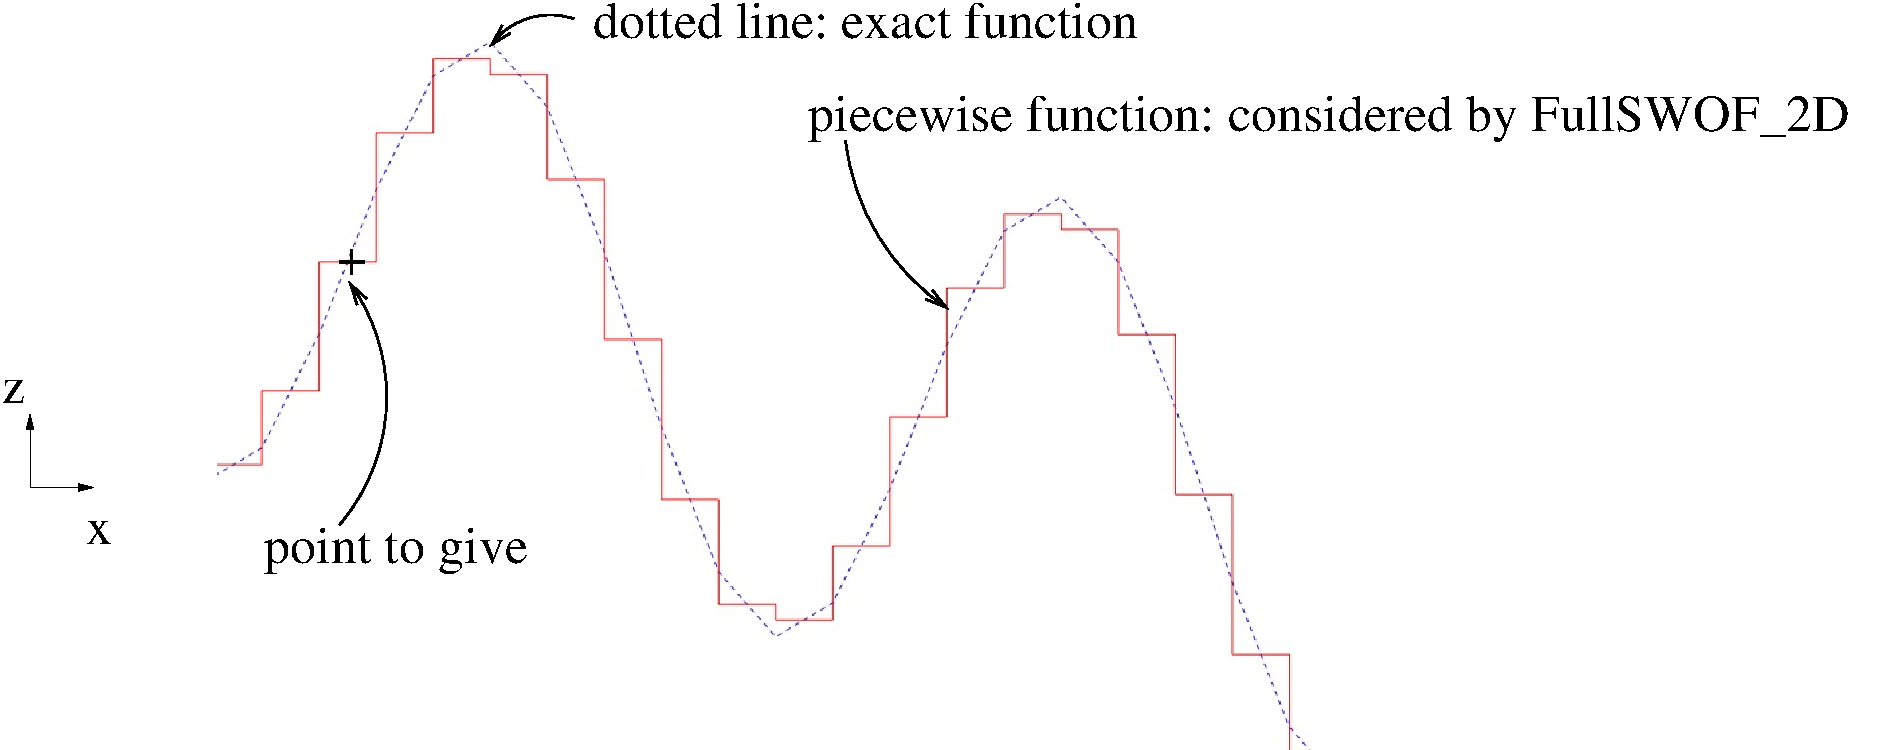
\includegraphics[width=0.8\textwidth]{Figures_FullSWOF_2D/points-cells_2D}
		\caption{Piece-wise approximation of 2D curves in \FullSWOF{}.}%
		\label{fig:cells}
	\end{center}
\end{figure}

\begin{figure}[htbp]
	\begin{center}
		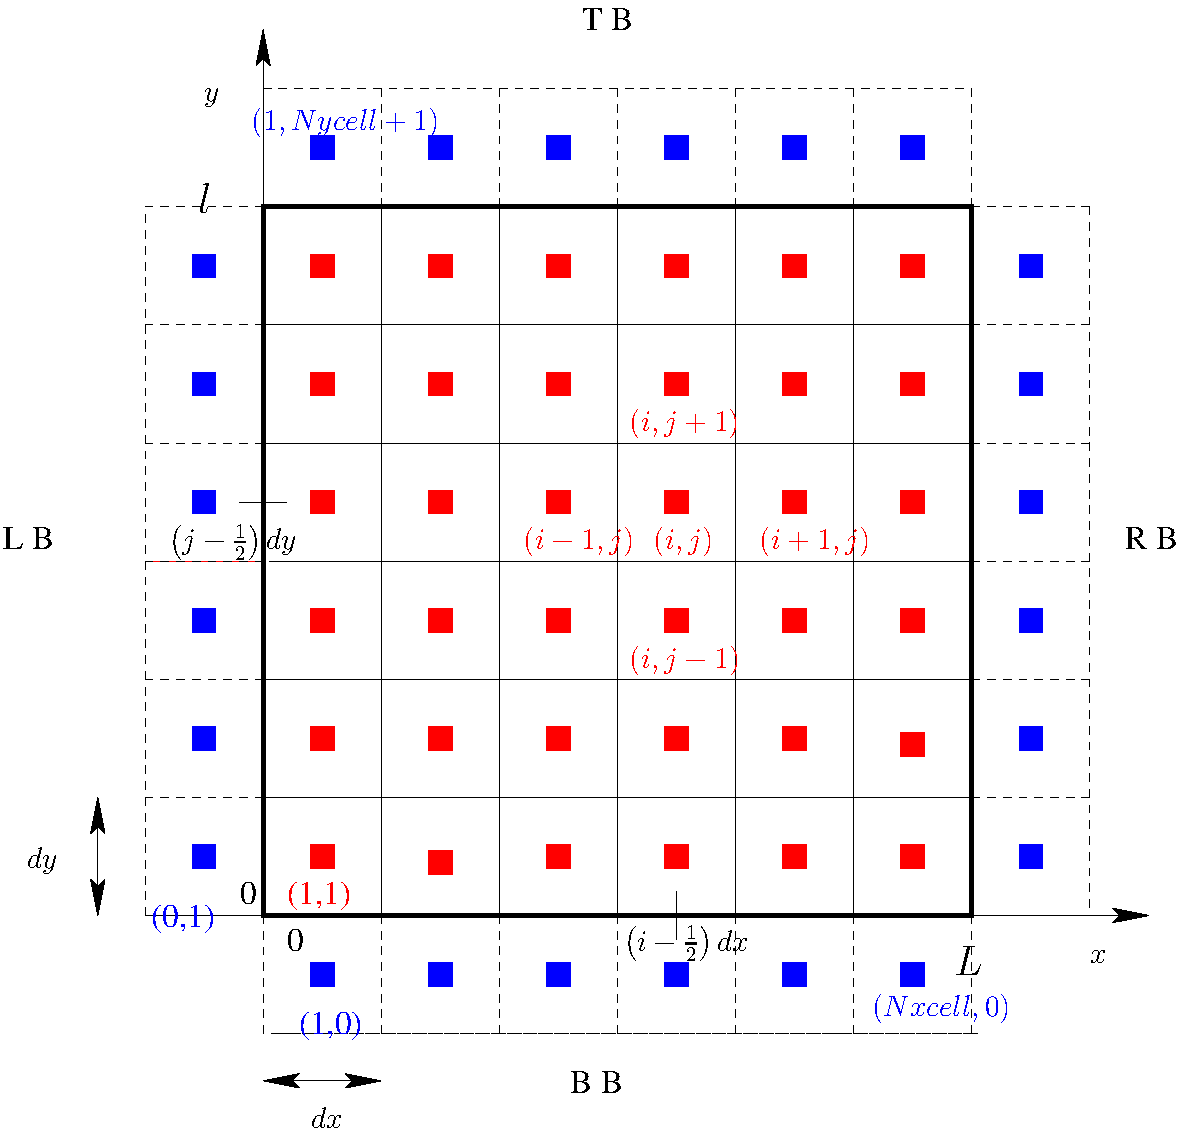
\includegraphics[width=12cm]{Figures_FullSWOF_2D/Maillage_FullSWOF_2D}
		\caption{Mesh of \FullSWOF.\newline
			LB= Left Boundary, RB= Right Boundary, BB= Bottom Boundary, TB= Top Boundary.\newline
			\textcolor{red}{The computational domain} is represented by the \textcolor{red}{cells with the red center} and the \textcolor{blue}{boundary} corresponds to \textcolor{blue}{the cells with blue center}.}%
		\label{fig:mesh}
	\end{center}
\end{figure}

\subsubsection{Initial water height and velocity}
You can impose the initial water height and velocity using \texttt{<huv\_init>}:
\begin{itemize}
	\item case~1 to load the initialization of variables \(h\)  [\si{\meter}], \(u\) [\si{\meter\per\second}] (velocity in the \(x\)-direction) and \(v\) [\si{\meter\per\second}] (velocity in the \(y\)-direction) from a file.
	      This file must be in ASCII and follow the format ``\(x\) \(y\) \(h\) \(u\) \(v\)''.
	      The \textbf{name of the file} \texttt{<huv\_NF>} should be specified and this file must be in the \textsf{Inputs} directory.
	\item case~2 to have \(h=\SI{0}{\meter}\), \(u=\SI{0}{\meter\per\second}\) and \(v=\SI{0}{\meter\per\second}\).
	\item case~3 to have the initialization for the paraboloid used as a benchmark in Section~\ref{ThackerParabBench}
	      and detailed in~\citet[§~4.2.2]{Delestre13}.\newline
	      You should choose the Thacker's topography for this case.
	\item case~4 to have \(h=\SI{0.005}{\meter}\) in a disk centered at (\(L/2,l/2\)) (which is the middle of the computation domain \([0;L] \times [0; l]\)) with a radius \(L/10\), \(h=\SI{0}{\meter}\) outside the disk, and \(u = v=\SI{0}{\meter\per\second}\) on the whole domain.
	      This case is used to simulate the dry radial dam break shown as a benchmark in Section~\ref{RadialDamDryBench} (Figure~\ref{fig:Radial_dam_dry}) and detailed in~\citet[§~4.1.2]{Delestre13}.
	      \newline
	      You should choose the flat topography for this case.
	\item case~5 to have \(h=\SI{0.005}{\meter}\) in a disk centered at (\(L/2,l/2\)) (which is the middle of the computational domain \([0;L] \times [0; l]\)) with a radius \(L/10\), \(h=\SI{0.001}{\meter}\) outside the disk, and \(u = v=\SI{0}{\meter\per\second}\) on the whole domain.
	      This case is used to simulate a wet radial dam (see Figure~\ref{fig:Radial_dam_wet}, and~\citet[§~4.1.1]{Delestre13}).\newline
	      You should choose the flat topography for this case.
\end{itemize}

\begin{figure}[htbp]
	\begin{center}
		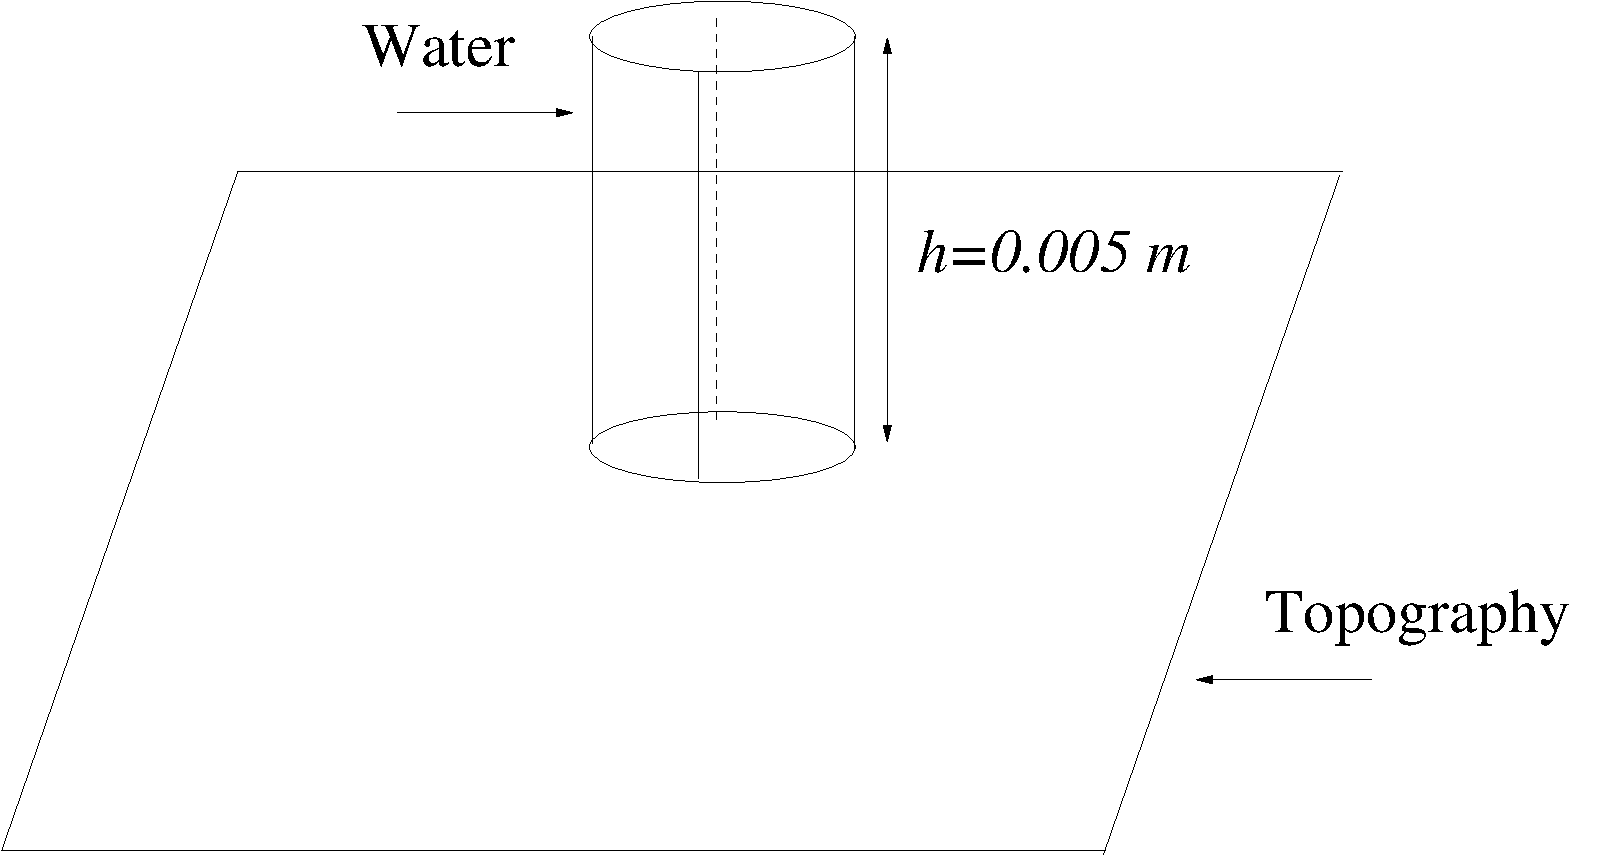
\includegraphics[width=0.8\textwidth]{Figures_FullSWOF_2D/Radial_dam_dry}
		\caption{Initialization of \(h\), \(u\) and \(v\) to simulate a dry radial dam:
			\(h=\SI{0}{\meter}\) or \(h=\SI{0.005}{\meter}\), \(u=\SI{0}{\meter\per\second}\), \(v=\SI{0}{\meter\per\second}\).}%
		\label{fig:Radial_dam_dry}
	\end{center}
\end{figure}

\begin{figure}[htbp]
	\begin{center}
		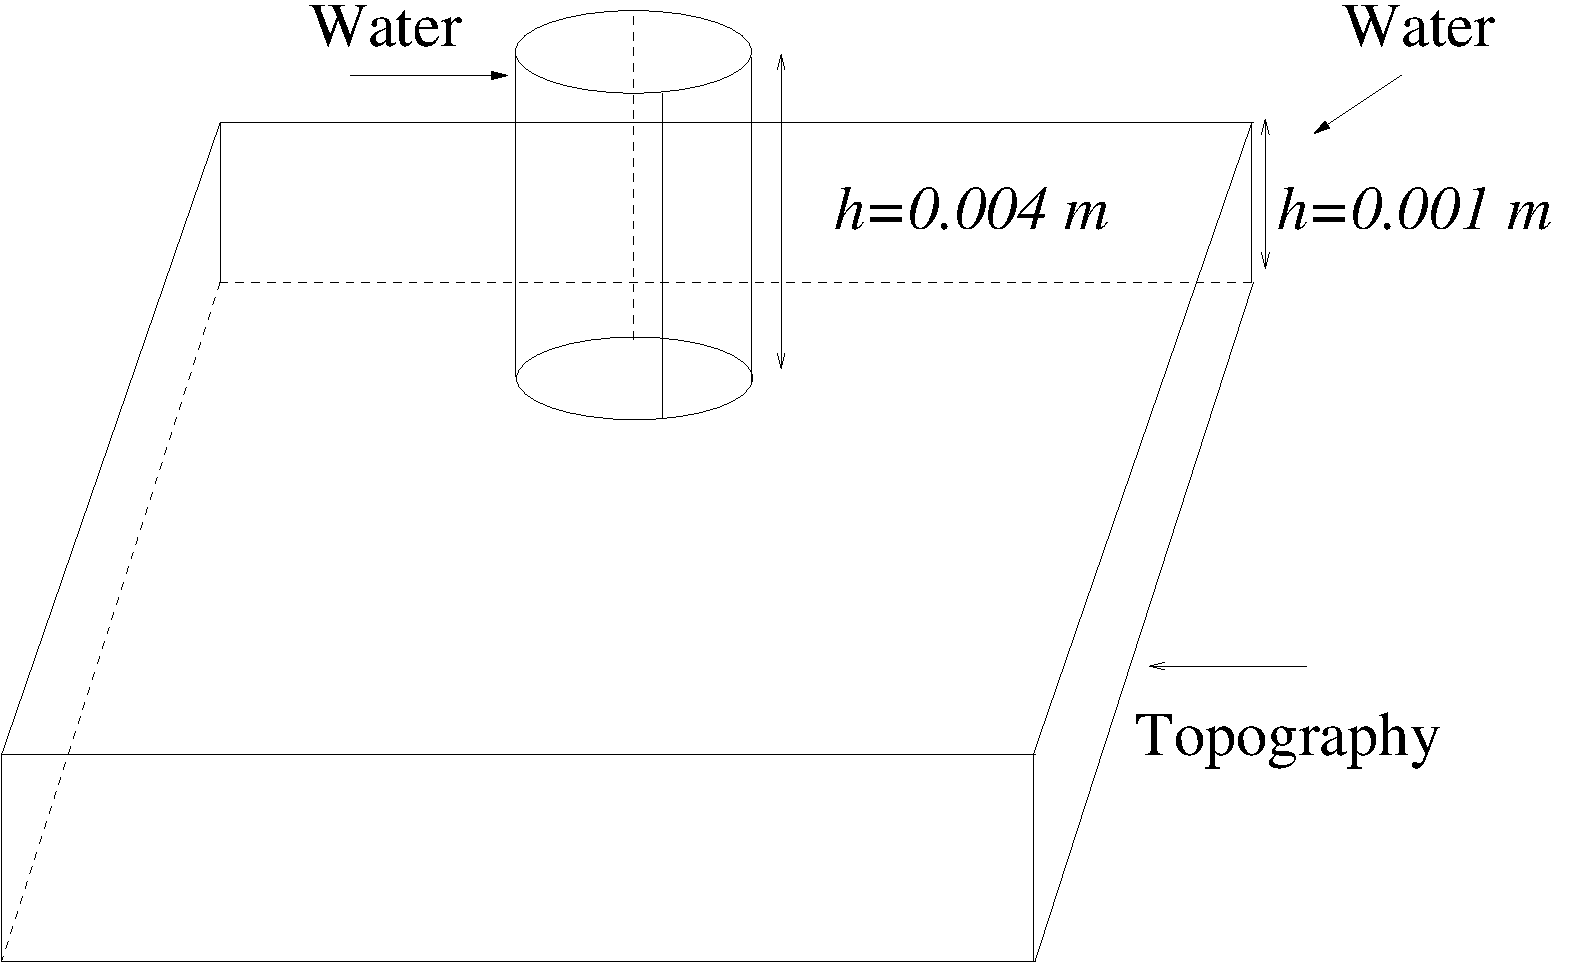
\includegraphics[width=0.8\textwidth]{Figures_FullSWOF_2D/Radial_dam_wet}
		\caption{Initialization of \(h\), \(u\) and \(v\)  to simulate a wet radial dam:
			\(h=\SI{0.001}{\meter}\) or \(h=\SI{0.005}{\meter}\), \(u=\SI{0}{\meter\per\second}\), \(v=\SI{0}{\meter\per\second}\).}%
		\label{fig:Radial_dam_wet}
	\end{center}
\end{figure}

\subsubsection{Rain}
For the \textbf{rain} \texttt{<rain>}, you can use:
\begin{itemize}
	\item case~0: \textbf{No Rain}.
	\item case~1: An ASCII file.
	      The \textbf{name of your rain file} \texttt{<rain\_NF>} should be set and this file must be in the \textsf{Inputs} directory.
	      \newline
	      The file must contain two columns (fig.~\ref{Fig:RainFile}):
	      \begin{itemize}
		      \item the first one represents the time [\si{\second}].
		      \item the second one the rain intensity [\si{\meter\per\second}].
	      \end{itemize}
	      Each column must contain at least one value.\newline
	      In the first column, the first value must be 0 (initial time).
	      If the file contains one line (namely 0 in the first column and any value in the second column), the rain intensity is constant during the run.\newline
	      If the file contains several lines with different values, the rain intensity will be changed during the simulation.
	      For example, let us consider three values for the time (\(0,t_1,t_2\)) and the corresponding three values for the rain intensity (\(a_0,a_1,a_2\)) (written into the second column).
	      Let us consider \(Rain(t)\) the intensity of the rain at the time t, we will get the values: \[Rain(t)=\left\{
		      \begin{array}{rl}
		      		{a_0} & \mathrm{for}\ 0 \leq t < t_1,   \\
		      		{a_1} & \mathrm{for}\ t_1 \leq t < t_2, \\
		      		{a_2} & \mathrm{for}\ t_2 \leq t.
		      \end{array}
		      \right.\]
	      \textbf{Be careful:} the intensity may not change exactly at \(t=t_1\) but at \(t>t_1\).
	      Indeed, whether using a constant CFL or a constant time step, \(t_1\) might not be reached exactly.
	      We can have \(t<t_1\) for a given computing step, and the next computing step (at \(t+dt\)) may be greater than \(t_1\).
	      So, \(t=t_1\) may not be computed.
	      In this case, the change in boundary condition will take place at \(t+dt>t_1\).

	      \begin{figure}[htpb]
		      \centering
		      \begin{tt}
			      \begin{tabular}{ll}
				      \#time & RainIntensity \\
				      0      & 0.001         \\
				      60     & 5e-4          \\
				      120    & 2e-5          \\
				      180    & 0
			      \end{tabular}
		      \end{tt}
		      \caption{Example of file for a rainfall evolving with time.\label{Fig:RainFile}}
	      \end{figure}

	\item case~2: the rain intensity is constant during the run.
	      The value is equals to \SI{e-5}{\meter\per\second} that is equivalent to \SI{36}{\milli\meter\per\hour}.
\end{itemize}
\begin{rmk}
	You can create another case from, for example, the function in the \textnormal{\textsf{rain\_generated.cpp}} file (see the  \textnormal{\textsf{Sources/librain\_infiltration}} directory).
\end{rmk}

\subsubsection{Name of output directory}

The default name of the output directory is \textsf{Outputs}.
However, you can add a \textbf{suffix} to this name (\texttt{<suffix\_o>}).
This is especially useful if you are running several tests.

\subsubsection{Format of the output files}

You have the choice between two possibilities to save the evolution of the computed values:
\begin{itemize}
	\item case~1: gnuplot format, designed for the gnuplot software (\url{http://www.gnuplot.info}).
	      This ASCII file can be used to draw easily the output using gnuplot software.
	\item case~2: vtk format can be used for the display of the computed values with Paraview software (\url{https://www.paraview.org}).
	      It is an ASCII file too.
\end{itemize}

\subsubsection{Saving specific points}

With this option, you can save the output values at specific points during the simulation.
Indeed, some points in your domain can be of high interest, and you can choose to follow the evolution of the flow at these points in more details.
To do so, you must first choose the number of specific points to want:
\begin{itemize}
	\item case~0: if you do not want to use this option.
	\item case~1: if you want to save only one point; then, specify in the following lines the coordinates along \(x\) \texttt{<x\_coord>} and \(y\) \texttt{<y\_coord>}.
	      These coordinates have to be a mesh point.
	\item case~2: if you want to save several points; save the list of the coordinates of the points (in two columns: \(x_i\) \(y_i\)) in an ASCII file, in the \textsf{Inputs} directory.
	      Give the \textbf{name of the file} \texttt{<list\_point\_NF>}.
\end{itemize}

You must also define the saving frequency.
You can choose either:
\begin{itemize}
	\item case~1: to save each time step.
	\item case~2: to set the interval between two savings.
	      In this case, you must specify the value of the time step in \texttt{<dt\_specific\_points>}.
\end{itemize}

For an example of using \FullSWOF{} with the saving of specific points, refer to the \textsf{Examples/Specific\_points} directory.

\subsubsection{Comments}
You can also add comments after the input value of each parameter.
For  example:\newline
\texttt{Time of simulation <T>:: 0.001 \# try 0.01 next time}

\subsubsection{Advised values}\label{rem:default}

For overland flow, several tests have been performed, in particular on the numerical scheme (see~\citet{Delestre10b}).
Consequently, we advise the user to choose by default the following numerical parameters:
\begin{itemize}
	\item \texttt{Choice of type of scheme (1=fixed cfl  2=fixed dt) <scheme\_type>:: 1}
	\item \texttt{Value of the cfl  <cflfix>:: 0.4}
	\item \texttt{Numerical flux (1=Rus 2=HLL 3=HLL2 4=HLLC 5=HLLC2) <flux>:: 5}
	\item \texttt{Order of the scheme <order>:: 2}
	\item \texttt{Reconstruction (1=MUSCL 2=ENO 3=ENOmod) <rec>:: 1}
	\item \texttt{Limiter (1=Minmod 2=VanAlbada 3=VanLeer) <lim>:: 1}
\end{itemize}

\medskip

If you choose the ENO or the modified ENO reconstruction, you should use:
\begin{itemize}
	\item \texttt{ENO damping factor <amortENO>:: 0.25}
	\item \texttt{Modified ENO factor <modifENO>:: 0.9}
\end{itemize}

\subsection{\textsf{Outputs} directory}\label{sec:outputs}

The results are saved in the \textsf{Outputs} directory.
When starting the program, the following files are saved:
\begin{description}
	\item[\textsf{parameters.dat}] contains the parameters used by \FullSWOF, under the same format as the input file.
	      In this file, the value of the parameters will be empty or equal to zero if the user did not fill them in \textsf{parameters.txt} file or if the value was not used.
	\item[\textsf{huz\_initial.dat}] contains the initial conditions (water height, velocity, topography and free surface).
\end{description}
During the computation, one file is modified in order to save several time steps:
\begin{description}
	\item[\textsf{huz\_evolution.dat}] contains the evolution (in time) of the main variables on each cell (water height, velocity, free surface, topography, the Euclidean norm of the velocity, Froude number, discharge along \(x\), discharge along \(y\), the Euclidean norm of the discharge).
	      There are \texttt{<nbtimes>} time steps saved.\newline
	      If you set \texttt{<nbtimes>} to 0, \FullSWOF{} will not create the \textsf{huz\_evolution.dat} file.
\end{description}

\medskip

If the computation is done until the final time, two other files are created:
\begin{description}
	\item[\textsf{huz\_final.dat}] contains the main variables on each cell (water height, velocity, free surface, topography, the Euclidean norm of the velocity, Froude number, discharge along \(x\), discharge along \(y\), the Euclidean norm of the discharge) at the final time.
	\item[\textsf{results.dat}] contains a mass balance to check the scheme conservation at the final time.
	      More precisely, you get:
	      \begin{itemize}
		      \item Infiltrated volume [\si{\cubic\meter}] is the total infiltrated water volume cumulated during the simulation.
		      \item Stream volume [\si{\cubic\meter}] is the total water volume staying at the final time above topography.
		      \item Complete volume (Inf+Stream) [\si{\cubic\meter}] is the sum of infiltrated volume and stream volume.
		      \item Volume of the rain [\si{\cubic\meter}] is the total rain volume cumulated during the simulation.
		      \item Outflow volume [\si{\cubic\meter}] is the sum of the cumulated outflow volume at all boundaries.
		      \item Duration of the computation [\si{\second}].
		      \item Number of iterations in the algorithm [\si{dimensionless}].
		      \item Mean Froude number [\si{dimensionless}] in space at the final time.
	      \end{itemize}
\end{description}

\medskip

If you chose to save one or more points during the simulation, \FullSWOF{} creates the file:
\begin{description}
	\item[\textsf{hu\_specific\_points.dat}] which contains the time in the first column and in the other columns the \(x\) and \(y\) coordinates selected by the user and the values of main variables (water height [\si{\meter}] and velocity [\si{\meter\per\second}]).\newline
	      Note that, in the case of several points, if you need to extract the evolution of only one point, the syntax of a \textsf{gawk} command is given in the header of the \textsf{hu\_specific\_points.dat} file.
\end{description}

\medskip

Finally, if you ran \FullSWOF{} in debug mode (see Section~\ref{sec:debug}), four other files are saved:
\begin{description}
	\item[\textsf{check\_vol.dat}] contains the cumulated volumes [\si{\cubic\meter}] at each time step.
	      The first column is the time and the others are: the overland flow volume (Vol\_of\_tot), the infiltrated volume (Vol\_inf\_tot), the rain volume (Vol\_rain\_tot) and the balance of the input and output volumes at the boundaries (Vol\_bound\_tot).
	\item[\textsf{boundaries\_flux.dat}] contains the cumulated fluxes [\si{\square\meter}] for each boundary and at each time step.
	\item[\textsf{flux\_boundaries\_LR.dat}] contains the fluxes [\si{\square\meter\per\second}] calculated at each cell of the left and right boundaries.
	\item[\textsf{flux\_boundaries\_BT.dat}] contains the fluxes [\si{\square\meter\per\second}] calculated at each cell of the bottom and top boundaries.
\end{description}

\begin{rmk}
	Recall that the second order is computed thanks to a prediction-correction method.
	Hence, when the code is run at the second order, two fluxes are used to perform one time step.
	In this case, the two values printed at \(t^n\) are the cumulated volumes associated with the two fluxes used to compute the values at \(t^{n+1}\).
\end{rmk}

\section{For developers}\label{sec:dvp}

\subsection{Make commands}\label{sec:make}
To make easier its use and development, \FullSWOF{} comes with a set of make commands:
\begin{description}
	\item[\textsf{make}] compiles \FullSWOF{} in release mode, 	\textit{i.e.}~with options speeding up the computations.
	\item[\textsf{make clean}] removes the intermediary files used to build the \FullSWOF{} release-mode binary.
	\item[\textsf{make benchref}] compiles \FullSWOF{} in benchmark mode, \textit{i.e.}~with options ensuring computation reproducibility, then run all the benchmarks, and, finally, check if there are differences between your outputs and the outputs of the main developers (see Section~\ref{sec:functionOK}).
	\item[\textsf{make cleanbenchref}] removes the files created by \textsf{make benchref}.
	\item[\textsf{make benchuser}] compiles \FullSWOF{} in benchmark mode, \textit{i.e.}~with options ensuring computation reproducibility, then run all the benchmarks, and, finally, check if there are differences between your current outputs and the outputs you computed earlier with \textsf{make benchref} (see Section~\ref{sec:perfo}).
	      It can be used, for example, if you made a change in the code that could affect the results (see Section~\ref{sec:perfo}).
	\item[\textsf{make cleanbenchuser}] removes the files created by \texttt{make benchuser}.
	\item[\textsf{make distclean}] removes all the files created by the above commands.
\end{description}

\begin{rmk}
	If you are on a multi-core machine, you can speedup the compilation and the benchmark computation by adding \textnormal{\textsf{-j N}} to your make command (where \textnormal{\textsf{N}} is the number of cores you want to use), like \textnormal{\textsf{make -j 4 benchuser}} for using up to 4~cores.
\end{rmk}

\subsection{Debugging}\label{sec:debug}

If you make some changes in \FullSWOF, you may need to debug your code.
The default configuration is the release mode.
To change it into debug mode, you must set the \texttt{DEBUG} value to \texttt{yes} in the \textsf{make\_config} file.
In that case, additional output files will be created to help you in your tests (see Section~\ref{sec:outputs}).

\subsection{Check for performances}\label{sec:perfo}

\sloppy
\FullSWOF{} comes with a set of test cases used for benchmarking (see Section~\ref{sec:valid}).
Each test case has its own directory, which should contain:
\begin{itemize}
	\item the analytic solution (file \textsf{analytic.dat}),
	\item the \FullSWOF{} input parameters (\textsf{Inputs} directory),
	\item the benchmark outcome as computed by the developers (file \textsf{comp\_STANDARD.dat}),
	\item the benchmark outcome as computed on your computer after installation (file \textsf{comp\_REFERENCES.dat}) --- see Section~\ref{sec:functionOK}.
\end{itemize}

After you modify \FullSWOF{} code, you may want to check if the performances are the same, have been degraded (a bug?), or have been improved, compared to the capabilities of the software after installation.
For this, simply run the command \textsf{make benchuser}.
This will first compute all the test cases (the results of the computation will be stored in the \textsf{Outputs} directories).
Then, the differences with the analytic solutions will be computed and, finally it will be checked if they are differences between your current run and the run upon installation.

If there is no difference, you should get the diagnosis ``Results are identical.''\ for each test case.
If differences are reported for one or more test cases, you may first want to look at the files \textsf{diff\_REF\_USER.dat} of the relevant test cases.
After the header (lines starting with the \# character), are listed a set of values:
\begin{description}
	\item[The first column identifies the variable.
	      ] DhSI stands for ``Differences in water height in international system unit'' (meter in the case of water height) while Dh\% stands for ``Differences in water height expressed as a percentage'' (taking as a reference the case Outputs\_REFERENCES).
	      Differences in velocity starts with ``Du'' and differences in water flux starts with ``Dq''.
	\item[The second column identifies the statistics for each variable.] First is given the number of differences that cannot be computed (``nbdiff==NaN''), probably because it involves a division by zero.
	      Then the number of differences equal to zero, larger than zero and smaller than zero.
	      Following are the minimum, maximum, mean and median values, and finally the \(L^1\), \(L^2\) and \(L^\infty\) norms.
	\item[The third column shows the absolute differences.]
	\item[The fourth column shows the relative differences (as a percentage),] taking as a reference the case Outputs\_REFERENCES\@.
\end{description}
So, you should be able to identify if the differences concern numerous values (or just a few), and if they are about water height, velocity or flux.
At this stage in the diagnosis, it may be time to dig further by comparing the content of the \textsf{Outputs} and \textsf{Outputs\_REFERENCES} directories:
\begin{itemize}
	\item First, check for unwanted differences in the \textsf{parameter.dat} files.
	\item Check that the initial data are identical (files \textsf{huz\_initial.dat}).
	\item Locate the differences in the final results by comparing the files \textsf{huz\_final.dat}.
	\item Eventually, compare the time evolution of these differences (files \textsf{huz\_evolution.dat}).
\end{itemize}
Based on this, you should be able to evaluate if the software results are as accurate, more accurate or less accurate than before.
Since each test case addresses specific flow conditions (see Section~\ref{sec:valid}), you should be able to build a rationale about which part of the simulation has been impacted, and, if required, which part of the source code is involved.

\subsection{Doxygen}

You may wish to add some functionalities to \FullSWOF{} to suit your needs.
Always comment the files, at the beginning of the file, using Doxygen syntax (\url{http://www.doxygen.org}).
Then, you will be able to create the Doxygen documentation of the whole code.
\begin{description}
	\item[HTML documentation.]
	      \sloppy In order to generate the Doxygen html file, the \textsf{Doxygen\_config\_file\_html} file is saved in the \textsf{doc} directory.
	      To run Doxygen, from the \FullSWOF{} directory, use the command:\newline \textsf{doxygen doc/Doxygen\_config\_file\_html}\newline Warning: Graphviz (\url{https://www.graphviz.org}) must be in your PATH to generate HTML diagrams.
	      If not, change the HAVE\_DOT parameter of the \textsf{Doxygen\_config\_file\_html} file.
	      In the \textsf{doc/html} directory, \textsf{index.html} is created.
	\item[PDF documentation.]
	      To generate the Doxygen PDF file (using \LaTeX{}), you must use the \textsf{Doxygen\_config\_file\_latex} file and compile the \textsf{.tex} file:\newline
	      \textsf{doxygen doc/Doxygen\_config\_file\_latex}\newline
	      \textsf{cd doc/latex}\newline
	      \textsf{make}\newline
	      In the \textsf{doc/latex} directory, \textsf{refman.pdf} is created.
\end{description}
Your version of Doxygen should be 1.8.7 or greater.

\begin{rmk}
	To simplify these operations, run the script \textnormal{\textsf{UpdateDateVersion.sh}} located in the \textnormal{\textsf{bin}} directory.
\end{rmk}

\section{Validation}\label{sec:valid}

This software has been validated using several analytic solutions and benchmarks from the literature, gathered in~\citet{Delestre13} and in the SWASHES software (\url{https://sourcesup.renater.fr/projects/swashes/}).
Some of them are already configured in the \textsf{Benchmarks} directory.

In this documentation, we recall the main characteristics of these tests, and give the results of \FullSWOF\@.

\subsection{Steady-state solutions}

In this section, we focus on a family of steady-state solutions, that are solutions satisfying:
\begin{equation*}
	\partial_t h=\partial_t u=\partial_t v=0.
\end{equation*}

\subsubsection{Emerged bump at rest}

Here we present a steady-state case (see~\citet[§~3.1.2]{Delestre13}) with a flat topography at the boundaries, no rain, no friction and no diffusion.
Initial conditions satisfy the hydrostatic equilibrium
\begin{equation}
	h+z=\mathit{Cst}\;\text{and}\;q=\SI{0}{\square\meter\per\second}.
	\label{hydeq}
\end{equation}
This solution tests the preservation of steady state and the boundary condition treatment.

For this case, we choose a domain of length \(L=\SI{25}{\meter}\) with a topography given by:
\begin{equation*}
	z(x,y) = \max\left(0\; , 0.2-0.05{(x-10)}^2-0.1{(y-10)}^2\right)
\end{equation*}
The water height is smaller than the topography height in order to have emergence of some parts of the bump.
In such a configuration, starting from the steady state, the velocity must remain null and the water surface should stay flat (see Figure~\ref{FigBumpemerged}).

\begin{figure}[htbp]
	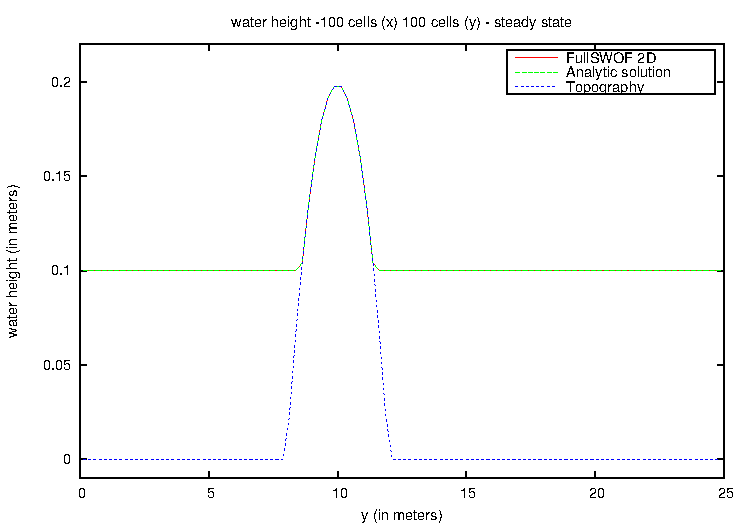
\includegraphics[width=0.48\textwidth]{Figures_FullSWOF_2D/Bump_emerged_Lake_at_rest_h}\ 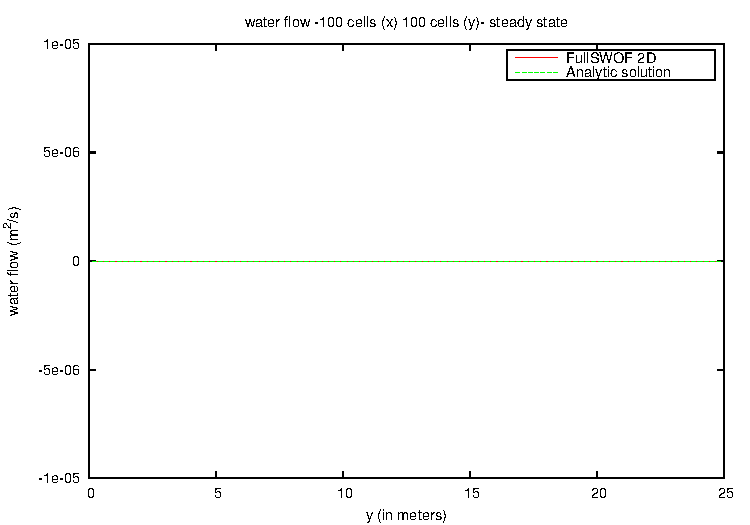
\includegraphics[width=0.48\textwidth]{Figures_FullSWOF_2D/Bump_emerged_Lake_at_rest_q}
	\caption{Emerged bump at rest}%
	\label{FigBumpemerged}
\end{figure}

\subsubsection{Fluvial Mac Donald test with rain and Darcy-Weisbach friction coefficient}

For a \SI{1000}{\meter} long channel, we consider a flow which is fluvial on the whole domain (see Figure~\ref{FigRain_flu} and~\citet[§~3.3.1]{Delestre13}).
Thus we impose a constant discharge (\(q=\SI{1}{\square\meter\per\second}\)) at the inflow and a constant water height at the outflow.\newline
Initially, the channel is dry and we choose Darcy-Weisbach friction law with \(f=0.093\).
We also impose a constant rain intensity (\(R_{0}=\SI{0.001}{\meter\per\second}\)) during the simulation.
%\begin{equation*}
% \left\{\begin{array}{l}
%   \text{upstream:}\;q=q_0,\\
%   \text{downstream:}\;h=h_{ex}(1000),
% \end{array}\right.
%\end{equation*}
%with the initial conditions
%\[ h = 0~\text{m} \mbox{ and } q=0~\text{m}^2/\text{s}.\]

%For the friction term, we have chosen Darcy-Weisbach's law with \(f=0.093\),
% the discharge \(q_{0}\) is set at \(1~\text{m}^2/\text{s}\) and the rain intensity is \(R_{0}=\SI{0.001}{\meter\per\second}\).

\begin{figure}[htbp]
	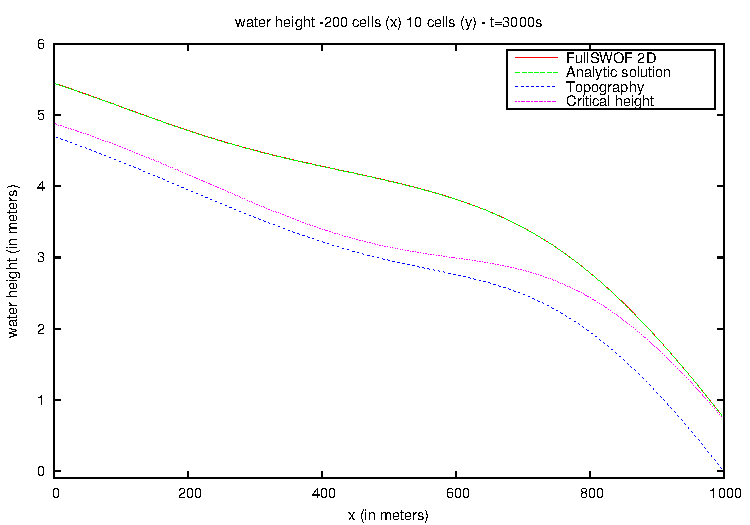
\includegraphics[width=0.48\textwidth]{Figures_FullSWOF_2D/MacDo_rain_flu_DW_h}\ 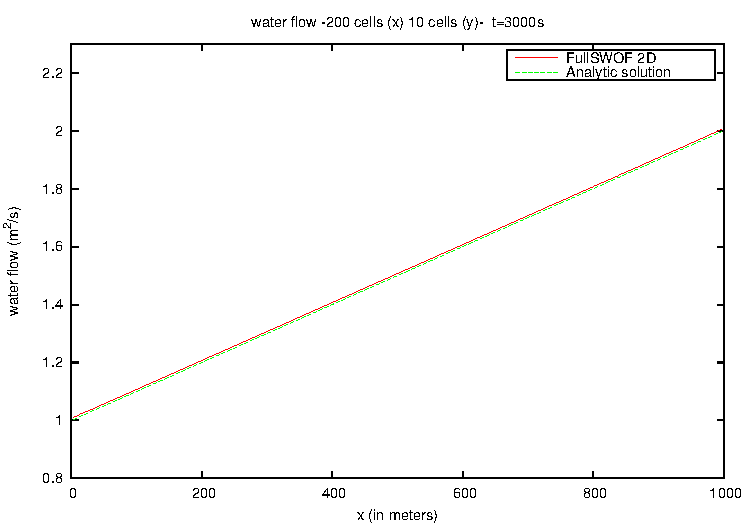
\includegraphics[width=0.48\textwidth]{Figures_FullSWOF_2D/MacDo_rain_flu_DW_q}
	\caption{Fluvial MacDonald Rain test with Darcy-Weisbach friction coefficient}%
	\label{FigRain_flu}
\end{figure}

\subsubsection{Torrential Mac Donald test with rain and Darcy-Weisbach friction coefficient}

The channel length remains unchanged (\SI{1000}{\meter}), but, as the flow is supercritical, we consider constant discharge (\(q=\SI{2.5}{\square\meter\per\second}\)) and water height at the inflow, and a free outflow (see Figure~\ref{FigRain_tor} and~\citet[§~3.3.1]{Delestre13}).
At initial time, the channel is dry and we choose Darcy-Weisbach friction law with \(f=0.065\).
\newline
%\begin{equation*}
% \left\{\begin{array}{l}
%   \text{upstream:}\;q = q_{0} \mbox{ and } h=h_{ex}(0),\\
%   \text{downstream: free.}
% \end{array}\right.
%\end{equation*}

%\[ h = 0~\text{m} \mbox{ and } q=0~\text{m}^2/\text{s}.\]

In this benchmark, there is no rain until \SI{1500}{\second} and after the rain intensity is \SI{0.0041}{\meter\per\second} until the end.
%The general form of the used rainfall event is
%\begin{equation*}
%R(t)=\left\{\begin{array}{ll}
%         0 \text{ m/s}    &  \text{if}\;t<t_{R},\\
%  R_{0}   &  \text{else},
%        \end{array}\right.
%\end{equation*}
%with \(t_{R} = 1500~.\\

%We have a friction coefficient \(f = 0.065\) for Darcy-Weisbach's law. Inflow
% discharge is \(q_0=2.5\;\text{m}^2/\text{s}\) and \(R_{0}=\SI{0.001}{\meter\per\second}\) (see Figure~\ref{FigRain_tor}).

\begin{figure}[htbp]
	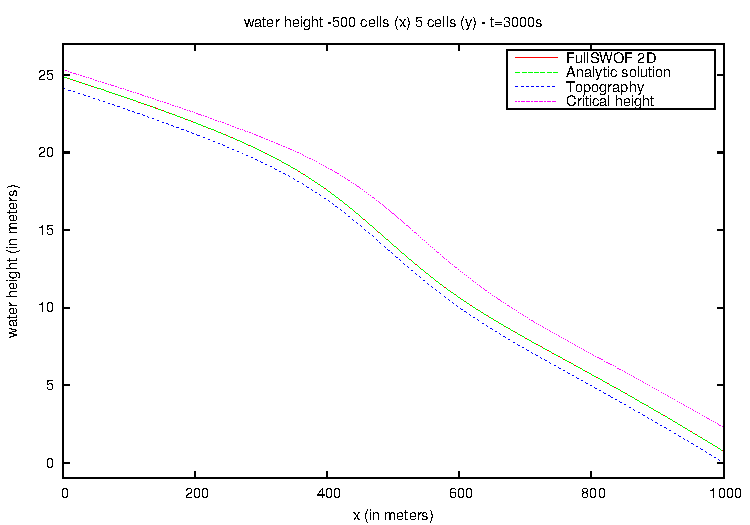
\includegraphics[width=0.48\textwidth]{Figures_FullSWOF_2D/MacDo_rain_tor_DW_h}\ 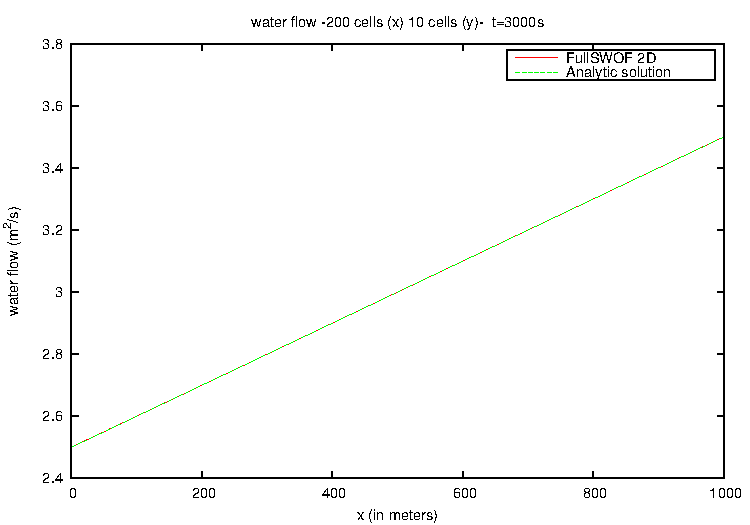
\includegraphics[width=0.48\textwidth]{Figures_FullSWOF_2D/MacDo_rain_tor_DW_q}
	\caption{Torrential MacDonald: Rain test with Darcy-Weisbach friction coefficient}%
	\label{FigRain_tor}
\end{figure}

\subsubsection{Mac Donald test with smooth transition and shock, with Manning friction coefficient}

The length of the channel is \SI{100}{\meter} and the discharge at steady state is \(q=\SI{2}{\square\meter\per\second}\).
The flow is fluvial both upstream and downstream (see Figure~\ref{FigMacDosmoothtrans} and~\citet[§~3.2.2]{Delestre13}).
In this case, the Manning friction coefficient is \(n = \SI{0.0328}{\metre\tothe{-1/3}\second}\), the inflow is subcritical, becomes supercritical via a sonic point, and, through a shock (located at \(x=200/3 \approx \SI{66.67}{\meter}\)), becomes subcritical again.

\begin{figure}[htbp]
	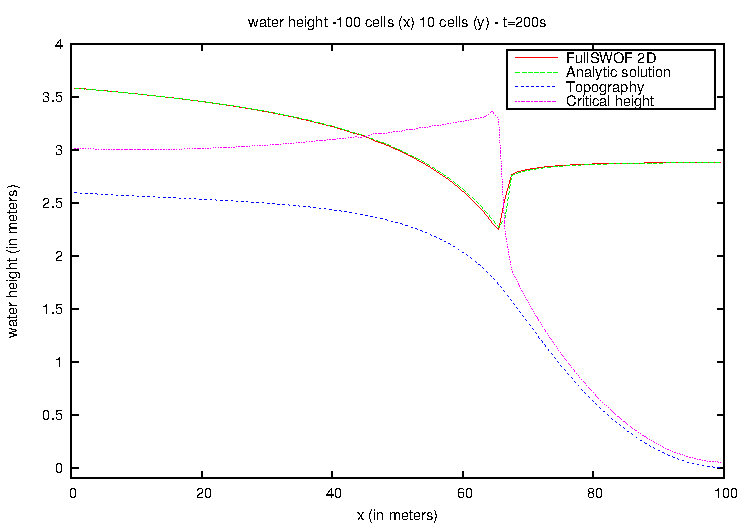
\includegraphics[width=0.48\textwidth]{Figures_FullSWOF_2D/MacDo_tor_flu_tor_Man_h}\ 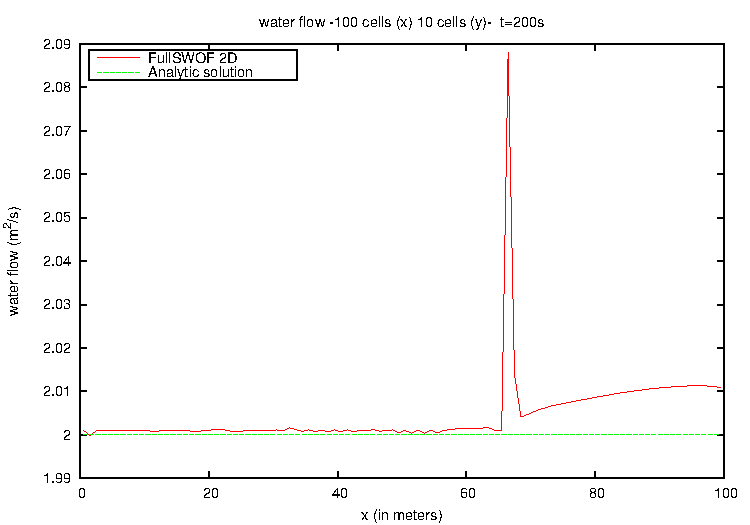
\includegraphics[width=0.48\textwidth]{Figures_FullSWOF_2D/MacDo_tor_flu_tor_Man_q}
	\caption{Mac Donald test with smooth transition and shock, with Manning friction coefficient}%
	\label{FigMacDosmoothtrans}
\end{figure}

\subsubsection{Mac Donald pseudo-2D solutions}
In this section, we give several analytic solutions for the pseudo-2D Shallow-Water system (see~\citet[§~3.5]{Delestre13}).
This system can be considered as an intermediate between the one-dimensional and the two-dimensional models.
More precisely, these equations model a flow in a rectilinear three-di\-men\-sional channel with the quantities averaged not only on the vertical direction but also on the width of the channel.

We consider two cases for non-prismatic channels.
Each channel is determined through the definition of the bottom width \(B\) (as a function of the space variable \(x\)) and the slope of the boundary \(Z\).
The bed slope is an explicit function of the water height.

\paragraph{Torrential Mac Donald pseudo-2D test with Manning friction coefficient}

In this case, the flow (\(q=\SI{20}{\cubic\meter\per\second}\)) and the water height are set at the inflow whereas the outflow is free (see Figure~\ref{Figpseudo2D_tor} and~\citet[§~3.5.2]{Delestre13}).\newline
The channel is initially dry and the flow is supercritical during the simulation.
% We have the following boundary conditions:
%\begin{equation*}
%  \left\{\begin{array}{l}
%     \text{upstream:}\;q=20\text{ m}^3 \text{s}^{-1}\; \text{and}\; h=h_{in},\\
%     \text{downstream: free.}
%  \end{array}\right.
%\end{equation*}

%The channel is initially dry, \emph{i.e.} initial conditions are:
%\begin{equation*}
%  h=0\text{ m},\;\text{and}\;q=0\;\text{m}^3/\text{s}.
%\end{equation*}

%In this case, the flow is supercritical.
\begin{figure}[htbp]
	\begin{center}
		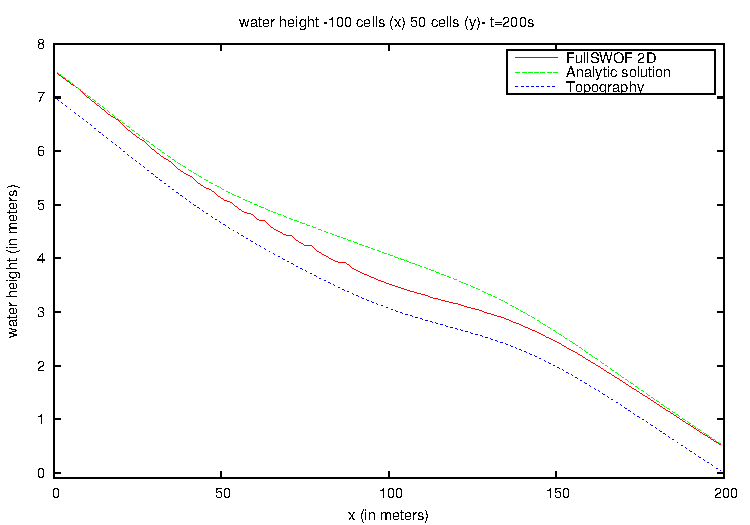
\includegraphics[width=0.48\textwidth]{Figures_FullSWOF_2D/MacDoP2D_tor_Man_h}
		\caption{Torrential Mac Donald  pseudo 2D test with Manning friction coefficient}%
		\label{Figpseudo2D_tor}
	\end{center}
\end{figure}

\paragraph{Fluvial Mac Donald pseudo-2D test with Manning friction coefficient}

Now, the length of the domain is \(L = \SI{400}{\meter}\), the boundaries of the channel are given by \(B_{2}\) and the cross sections are isoscele trapezoids (see Figure~\ref{Fig:pseudo2D:b2} and~\citet[§~3.5.5]{Delestre13}).

In this case, the channel is initially dry, with a little puddle downstream.
The flow is imposed at the inflow (\(q=\SI{20}{\cubic\meter\per\second}\)) and the water height is prescribed at the outflow (see Figure~\ref{Fig:pseudo2D:fluMan}).
The flow is subcritical along the whole channel.

% We have the following boundary conditions:
%\begin{equation*}
%  \left\{\begin{array}{l}
%     \text{upstream:}\;q=20\text{ m}^3 \text{s}^{-1},\\
%     \text{downstream:}\;h=h_{out}.
%  \end{array}\right.
% \end{equation*}

\begin{figure}[htbp]
	\begin{subfigure}[b]{0.5\textwidth}
		\centering
		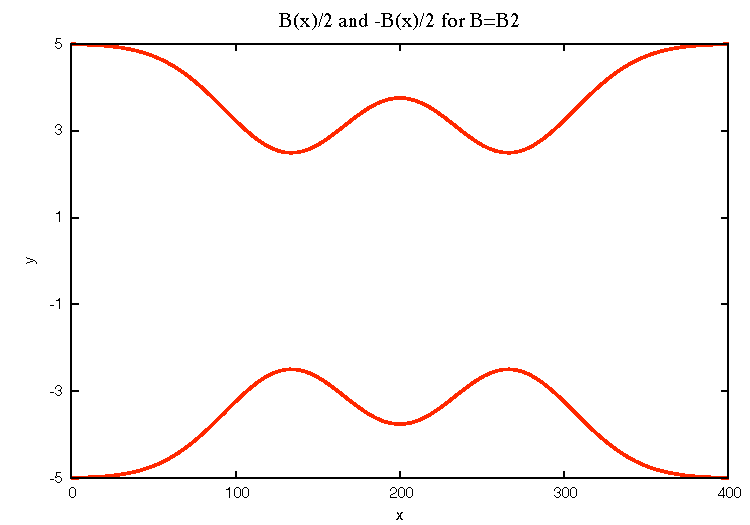
\includegraphics[width=\textwidth]{Figures_FullSWOF_2D/MacDonald_b2}
		\caption{Function B2 for the shape of the channel.}%
		\label{Fig:pseudo2D:b2}
	\end{subfigure}
	%
	\begin{subfigure}[b]{0.5\textwidth}
		\centering
		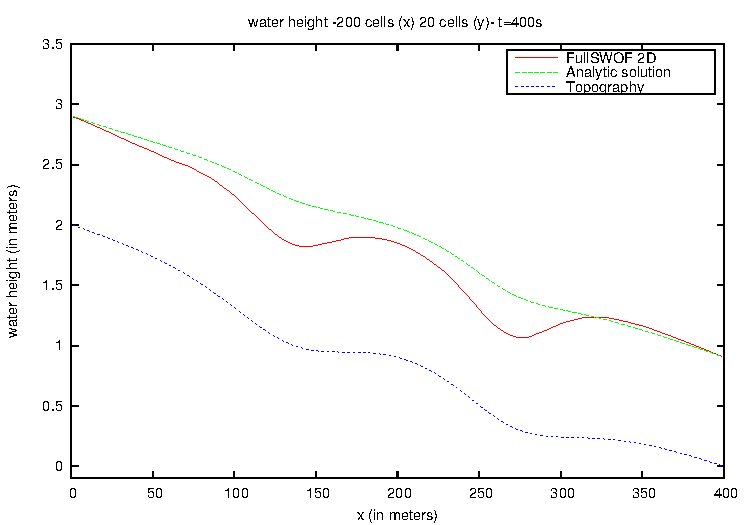
\includegraphics[width=\textwidth]{Figures_FullSWOF_2D/MacDoP2D_flu_Man_h}
		\caption{Simulation results}%
		\label{Fig:pseudo2D:fluMan}
	\end{subfigure}
	\caption{The fluvial Mac Donald pseudo-2D test with Manning friction coefficient\label{Fig:pseudo2D}}
\end{figure}

\subsection{Transitory solutions}

In the previous section, we gave steady-state solutions of increasing difficulties.
These solutions can be used to check if the numerical methods are able to keep/catch steady-state flows.
But even if the initial condition differs from the expected steady-state, we do not have information about the transitory behavior.
Thus, in this section, we give some transitory solutions that may improve the validation of the numerical methods.
Moreover, as these cases have wet/dry transitions, one can check the ability of the schemes to capture the evolution of these fronts (\emph{e.g.} some methods may fail and give negative water height).
At last, we give a periodic transitory solution in order to check whether the schemes are numerically diffusive or not.

\subsubsection{Dam break on a dry domain without friction}\label{RadialDamDryBench}

In this section, we are interested in a dam break solution on a flat topography namely Ritter's solution (see~\citet[§~4.1.2]{Delestre13}).
The initial condition for this configuration is the following Riemann problem
	\[h(x,y)=
	\begin{cases}
		\SI{0.005}{\meter} & \mathrm{for}\ \SI{0}{\meter}\leq y \leq L-x , \\ \SI{0}{\meter} & \mathrm{for}\ y > L-x,
	\end{cases}
	\] with \(u(x,y)=v(x,y)= \SI{0}{\meter\per\second}\).
The comparison between the solution given by \FullSWOF{} and analytic solution is shown in Figure~\ref{FigDambreak}.

\begin{figure}[htbp]
	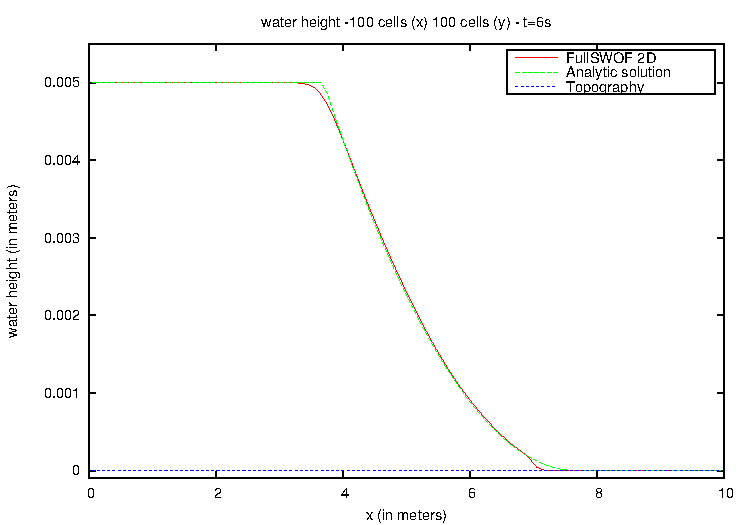
\includegraphics[width=0.48\textwidth]{Figures_FullSWOF_2D/Dry_Dam_Break_h}\ 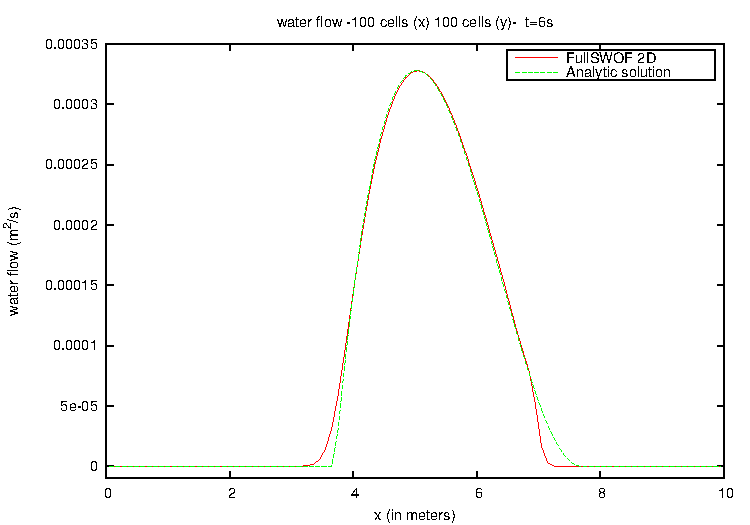
\includegraphics[width=0.48\textwidth]{Figures_FullSWOF_2D/Dry_Dam_Break_q}%
	\caption{Dam break dry without friction}%
	\label{FigDambreak}
\end{figure}

\subsubsection{Thacker test case with planar surface in a paraboloid}\label{ThackerParabBench}

For this Thacker 2D case, the moving shoreline is a circle and the topography is a paraboloid of revolution.
The free surface has a periodic motion and remains planar in time (see~\citet[§~4.2.2]{Delestre13}).
To visualize this case, one can think of a glass with some liquid in rotation inside (see Figure~\ref{FigThacker}).

Here again, the analytic solution at \(t=\SI{0}{\second}\) is taken as initial condition.
This is an analytic solution with a variable slope (in space) for which the wet/dry transitions are moving.
It also tests the ability of the schemes to simulate flow with comings and goings and, as the water height is periodic in time, the numerical diffusion of the scheme.
\begin{figure}[htbp]
	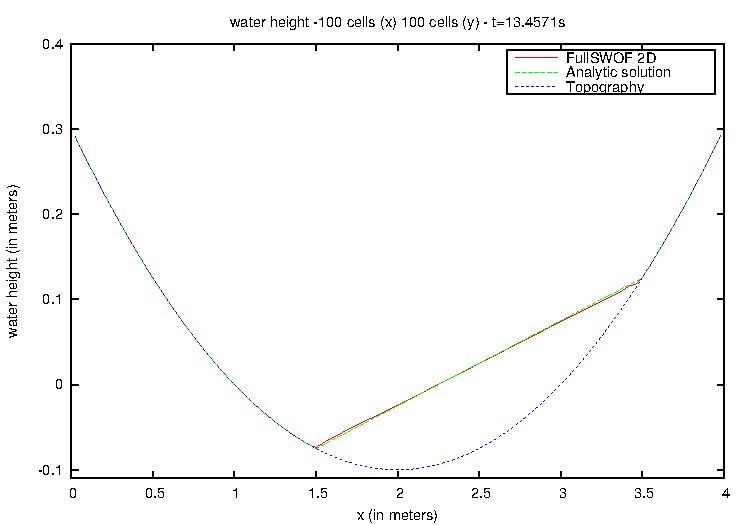
\includegraphics[width=0.48\textwidth]{Figures_FullSWOF_2D/Thacker_planar_h}\ 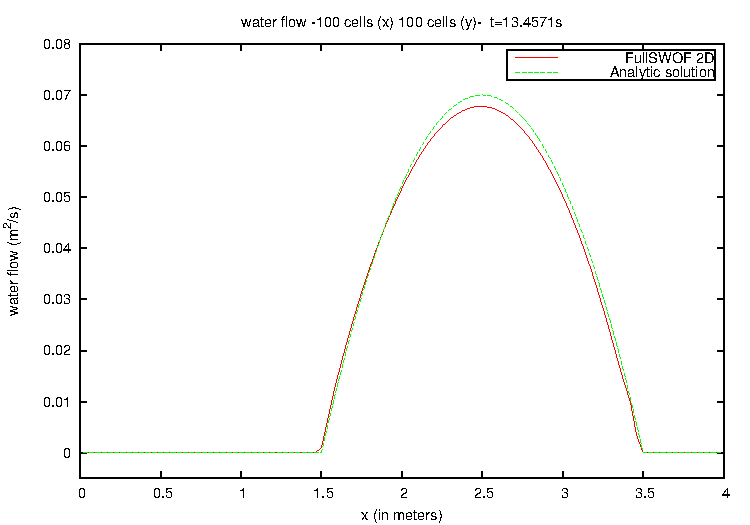
\includegraphics[width=0.48\textwidth]{Figures_FullSWOF_2D/Thacker_planar_q}%
	\caption{Thacker test case with planar surface in a paraboloid}%
	\label{FigThacker}
\end{figure}

\bibliographystyle{apalike-refs}
\bibliography{doc}

\end{document}
